\section{Introduction}

Visual anomaly detection (VAD) is a prerequisite for safety in manufacturing quality control, medical imaging, infrastructure inspection, and autonomous driving.
Recent work has explored using vision-language models (VLMs) for anomaly detection, either via task-specific tuning or via zero-shot reasoning over image content in natural language~\citep{gu2024anomalygpt,jiang2024mmad,chen2026eagle}.
Yet three fundamental limitations prevent VLMs from serving as reliable anomaly detectors across diverse domains.

\paragraph{Three common VLM limitations in VAD.}
\emph{(1) Lack of quantitative grounding.}
VLMs reason about visual content in natural language but cannot compute the patch-level distance statistics that make expert detectors like PatchCore~\citep{roth2022patchcore} effective.
When a subtle surface scratch changes patch distances by 0.15 standard deviations, the VLM sees only pixels and may miss it entirely.
\emph{(2) Hallucination and under-detection.}
Without quantitative anchoring, VLMs hallucinate defects on unfamiliar but normal images (e.g., benign liver cysts flagged as lesions) or fail to detect genuine anomalies when they lack domain-specific visual priors~\citep{jiang2024mmad}.
\emph{(3) Domain-blind calibration.}
A patch-level expert score of 0.3 is highly abnormal for industrial surfaces but entirely normal for medical tissue.
VLMs have no mechanism to interpret the same quantitative signal differently across domains.

Existing approaches address these limitations in isolation.
\emph{Vision-expert} methods~\citep{roth2022patchcore,oquab2024dinov2,jeong2023winclip} provide precise patch-level scores but cannot handle semantic or logical anomalies.
\emph{VLM-only} methods~\citep{gu2024anomalygpt,jiang2024mmad,cao2025anomalyonevision} reason fluently but lack quantitative grounding.
Recent tool-augmented approaches~\citep{zhang2025agentiad,chen2026eagle,wei2025autoiad} combine VLMs with expert tools, but communicate expert signals through visual overlays, require costly fine-tuning, or are evaluated only on industrial benchmarks.
Whether a single expert--VLM integration strategy can generalize across domains with fundamentally different anomaly semantics remains an open question.

\paragraph{Our approach.}
AnomaClaw resolves these limitations with a simple design principle: \emph{expert as context, not as decision-maker}.
Rather than routing queries to vision experts or fusing their scores with VLM predictions, we provide the expert's patch-level analysis as structured text to the VLM.
Concretely, a PatchCore-style module computes patch distances against a normal reference bank and produces a structured text summary (e.g., ``Patch-level anomaly score: 0.391; global similarity: 0.812; assessment: strong anomaly signal'').
The VLM receives this summary alongside DINOv2-retrieved reference images and the query image, retaining full decision authority while being grounded by quantitative evidence it could not compute on its own.
This design directly addresses the first VLM limitation by providing quantitative grounding, and partially mitigates the second by anchoring VLM decisions in measurable patch statistics.
The third limitation is addressed separately through an optional family-adaptive fusion step that calibrates the expert--VLM balance per domain type.
Matched ablations confirm that expert-as-context outperforms routing by 3.3 AUROC points and score fusion by 3.0 points.
The gain is largest on local-appearance domains where patch distances are most discriminative; on medical domains, the VLM can selectively discount expert evidence when it conflicts with clinical semantics.

\begin{figure}[t]
    \centering
    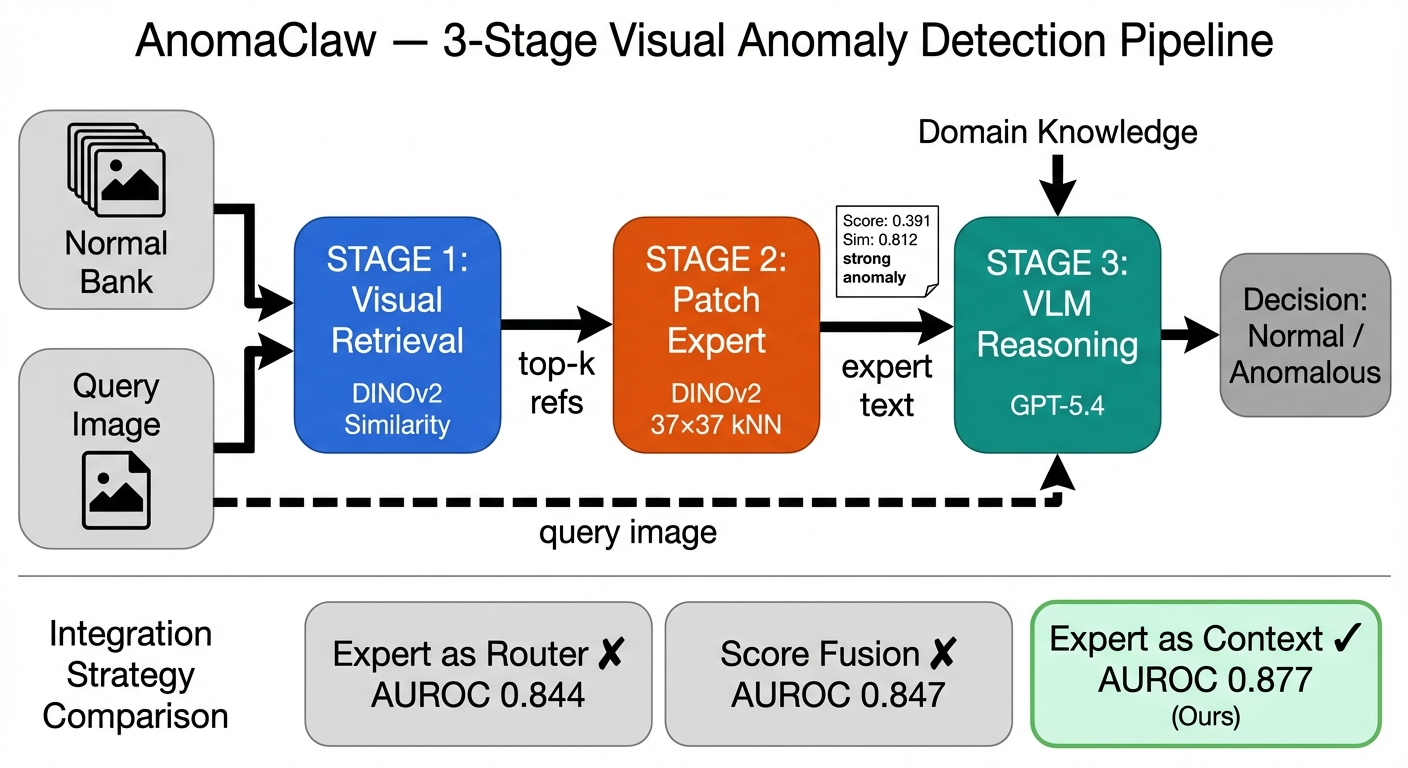
\includegraphics[width=0.95\linewidth]{figures/architecture.png}
    \caption{%
        \textbf{AnomaClaw overview.}
        Stage~1: DINOv2 retrieves the most similar normal references from a domain-specific bank.
        Stage~2: a PatchCore-style expert computes patch-level distances and emits a structured text summary.
        Stage~3: the VLM receives the query image, retrieved references, and the expert summary as text context, making the final anomaly decision.
        Bottom panel compares the expert-as-context design (ours) against expert-as-router and score-fusion alternatives.
    }
    \label{fig:overview}
\end{figure}

\paragraph{Contributions.}
Our main contributions are as follows:
\begin{enumerate}[leftmargin=*,itemsep=2pt,topsep=3pt]
    \item \textbf{Expert-as-context design principle.}
    Through matched ablations on identical backbones and data, we demonstrate that providing patch-level expert evidence as structured text context to VLMs outperforms expert-as-router (+3.3 AUROC points) and score-fusion (+3.0 points) integration strategies.
    This design provides quantitative grounding that VLMs cannot compute independently, while preserving their semantic reasoning authority.

    \item \textbf{Cross-domain VAD benchmark.}
    We assemble a unified evaluation spanning 10 domains---industrial surface inspection, retail product checking, concrete crack detection, dermatology, brain MRI, liver CT, gastrointestinal endoscopy, road safety, logical anomaly, and industrial functional inspection---comprising 1{,}200 test items plus a disjoint 200-item calibration split with standardized metrics and protocols.
    This benchmark reveals failure modes that domain-specific evaluations miss.

    \item \textbf{Family-adaptive fusion.}
    We introduce a calibration scheme that adapts the expert--VLM integration per domain family using a disjoint 200-item held-out split, achieving \textbf{0.882 macro AUROC} across all 10 domains---surpassing a pure VLM baseline (0.866) and a multi-round agent baseline (0.873)~\citep{zhang2025agentiad}.

    \item \textbf{Two operating points.}
    We characterize AnomaClaw under two deployment regimes: \emph{best accuracy} (0.882 AUROC, 100\% VLM calls) and \emph{best efficiency} (0.847 AUROC with only 41\% VLM calls, yielding a 59\% cost reduction), enabling practitioners to select the appropriate trade-off for their application.
\end{enumerate}

The remainder of the paper is organized as follows.
Section~\ref{sec:related} reviews VLM-based and expert-based anomaly detection.
Section~\ref{sec:method} details the AnomaClaw architecture.
Section~\ref{sec:setup} describes the cross-domain benchmark construction.
Section~\ref{sec:experiments} presents experiments and ablations, and Section~\ref{sec:conclusion} concludes.
